%%%%%%%%%%%%%%%%%%%%%%%%%%%%%%%%%%%%%%%%%
%
% (c) 2022 by Jennifer Laaser
%
% This work is licensed under the Creative Commons Attribution-NonCommercial-ShareAlike 4.0 International License. To view a copy of this license, visit http://creativecommons.org/licenses/by-nc-sa/4.0/ or send a letter to Creative Commons, PO Box 1866, Mountain View, CA 94042, USA.
%
% The current source for these materials is accessible on Github: https://github.com/jlaaser/pogil-polymers
%
%%%%%%%%%%%%%%%%%%%%%%%%%%%%%%%%%%%%%%%%%

\renewcommand{\figpath}{content/polymphys/thermal-transitions/thermal-characterization/figs}
\renewcommand{\labelbase}{thermal-characterization}

\begin{activity}{Measuring $T_g$ and $T_m$}

\begin{instructornotes}
	This activity introduces students to concepts related to measuring the glass transition temperatures and melting temperatures of polymer materials.
	
	After completing this activity, students will be able to:
	\begin{enumerate}
		\item ...
	\end{enumerate}
	
	\subsection*{Activity summary:}
	\begin{itemize}
		\item \textbf{Activity type:} Learning Cycle
		\item \textbf{Content goals:} Glass Transitions of Polymer Materials
		\item \textbf{Process goals:} %https://pogil.org/uploads/attachments/cj54b5yts006cklx4hh758htf-process-skills-official-pogil-list-2015-original.pdf
			\begin{enumerate}
				\item Linking concepts to derive a key result
				\item Communication (written and oral) of reasoning
			\end{enumerate}
		\item \textbf{Duration:} TBD
		\item \textbf{Instructor preparation required:} none beyond knowledge of relevant content
		\item \textbf{Related textbook chapters:}
			\begin{itemize}
				\item \emph{Polymer Chemistry} (Hiemenz \& Lodge): section XYZ
			\end{itemize}
		\item \textbf{Instructor notes:}
			\begin{itemize}
				\item \dots
			\end{itemize}
	\end{itemize}
	
\end{instructornotes}



\begin{model}[Dynamic Mechanical Analysis]
	\label{\labelbase:mdl:DMA}
	
	One common method for determining the $T_g$ and $T_m$ of a polymer material is to measure its modulus of the material as a function of temperature.
	
	Typically, these measurements are performed using either small-amplitude oscillatory shear rheology or dynamic mechanical analysis (DMA) performed at a constant oscillation frequency, typically 1 rad/s.
	
\end{model}


\begin{ctqs}

	\question How do you expect the storage modulus of a polymer sample to change as...
	
		\begin{enumerate}
			\item ... the temperature is increased from below $T_g$ to above $T_g$?
			
				\begin{solution}[0.75in]
				\end{solution}
			
			\item ... the temperature is further increased from below $T_m$ to above $T_m$?
			
				\begin{solution}[0.75in]
				\end{solution}
		
		\end{enumerate}
		
	\question Sketch the curve that you would expect to obtain in a measurement of $G'$ as a function of temperature for a polymer that has \emph{both} a glass transition \emph{and} a melting transition:
	
		\vspace{6pt}
		\centerline{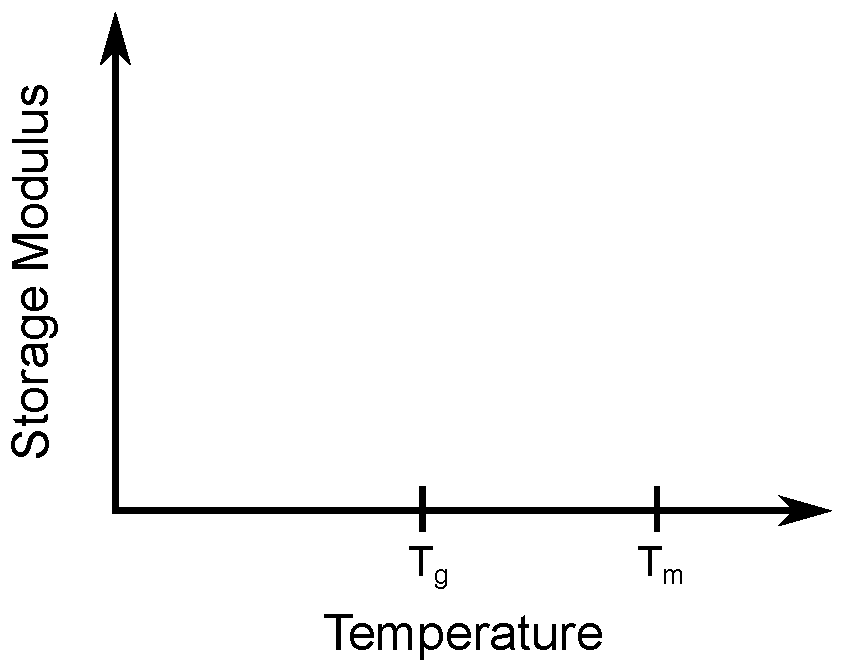
\includegraphics[width=0.5\textwidth]{\figpath/Model2_modulus_blank}}
		
	
	\clearpage
	\question The modulus of a sample of polycarbonate, measured by DMA, is shown below:
	
		\vspace{6pt}
		\centerline{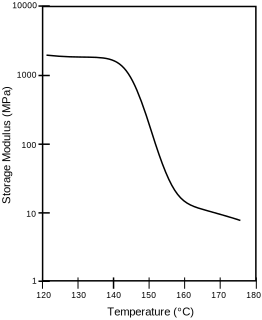
\includegraphics[width=0.35\textwidth]{\figpath/Model1_polycarbonateDMA}}
		
		What value would your group report as the glass transition temperature of this material?  Briefly explain your reasoning in 1-2 complete sentences.
		
		\begin{solution}[1in]
		\end{solution}
	
\end{ctqs}

%begin{infobox}
	
%	Often, it is easier to locate the glass transition by looking for either (i) a peak in the loss modulus, or (ii) a peak in the ratio of the storage and loss moduli (also referred to as $\tan\delta$).
	
%\end{infobox}

% would like to add a few CTQs getting at the idea that the peak in E'' occurs at the temperature at which the relaxation time is approx 1 s, but I think this requires more knowledge of the Maxwell Model than my students will realistically have

% could also turn into an exercise - maybe even get at the fact that you measure different Tg's with different deformation frequencies?

\begin{model}[Differential Scanning Calorimetry]
	
	Another common method for measuring $T_g$ and $T_m$ is \emph{differential scanning calorimetry} (DSC).  In a DSC experiment, the sample is heated at a constant rate, and the instrument measures the amount of heat (relative to a ``blank'' reference sample) that needs to be put in to maintain this constant rate of heating.
	
	For a sample with a constant heat capacity, a DSC experiment yields a flat line, as shown below:
	
		\centerline{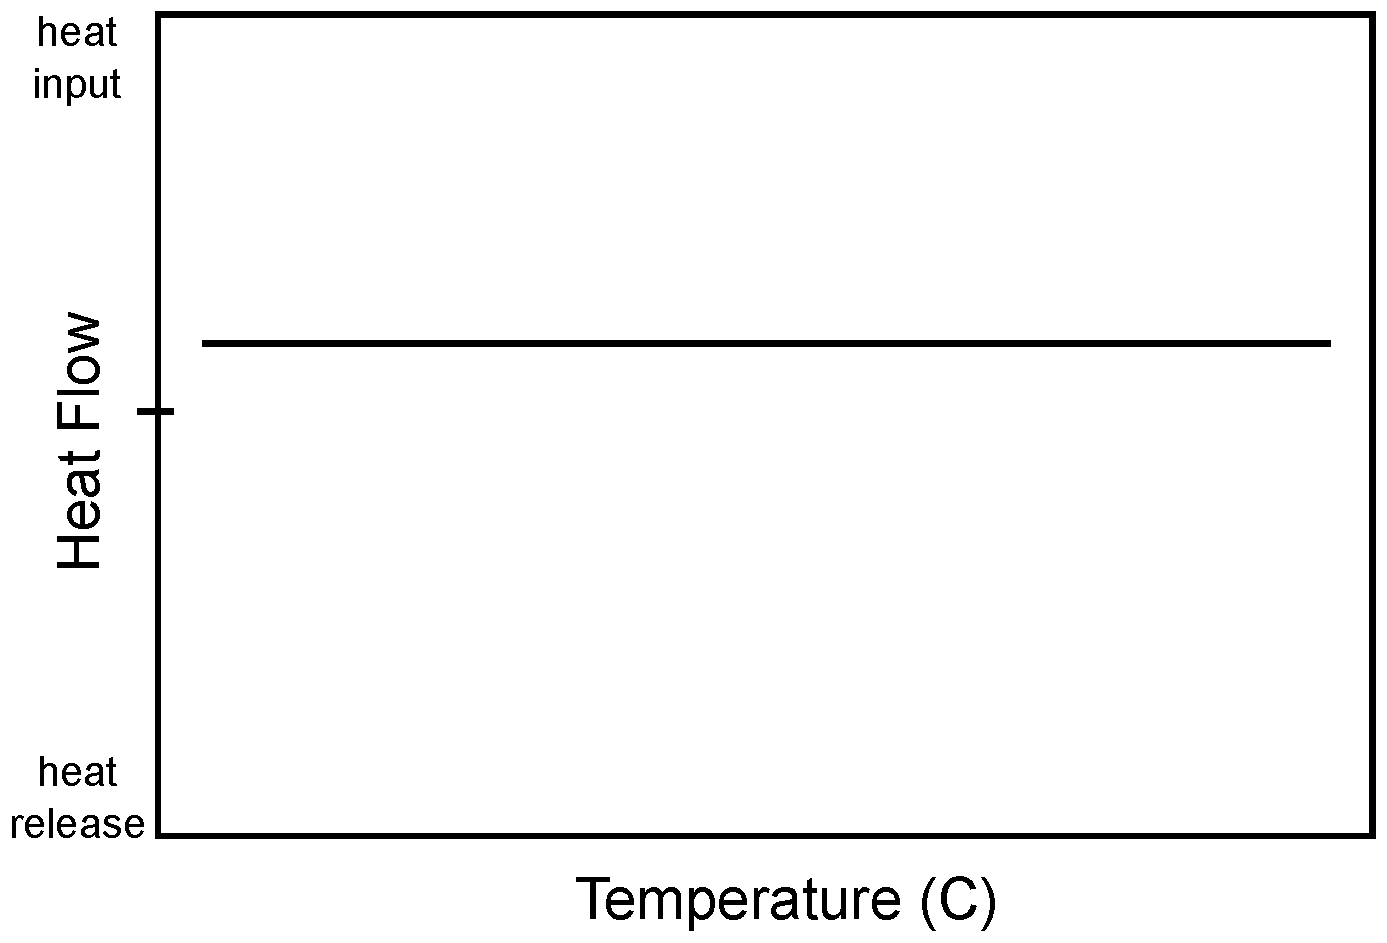
\includegraphics[width=0.5\textwidth]{\figpath/Model2_constCp}}
	
\end{model}

\begin{ctqs}

	\question Recall that the heat capacity of a material, $C_P$, is defined by
		\begin{equation*}
			C_p = \left(\frac{\partial H}{\partial T}\right)_P
		\end{equation*}
		Explain, in 1-2 complete sentences, why a material with constant $C_p$ gives a flat line in DSC.
		
			\begin{solution}[1.25in]
			\end{solution}
		
	\question Suppose that a material's heat capacity increases (from $C_{p,1}$ to $C_{p,2}$) at some temperature $T_0$.  What shape would you expect the resulting DSC curve to have?  Sketch your group's answer on the axes below: \label{\labelbase:ctq:CPincrease}
	
		\vspace{6pt}
		\centerline{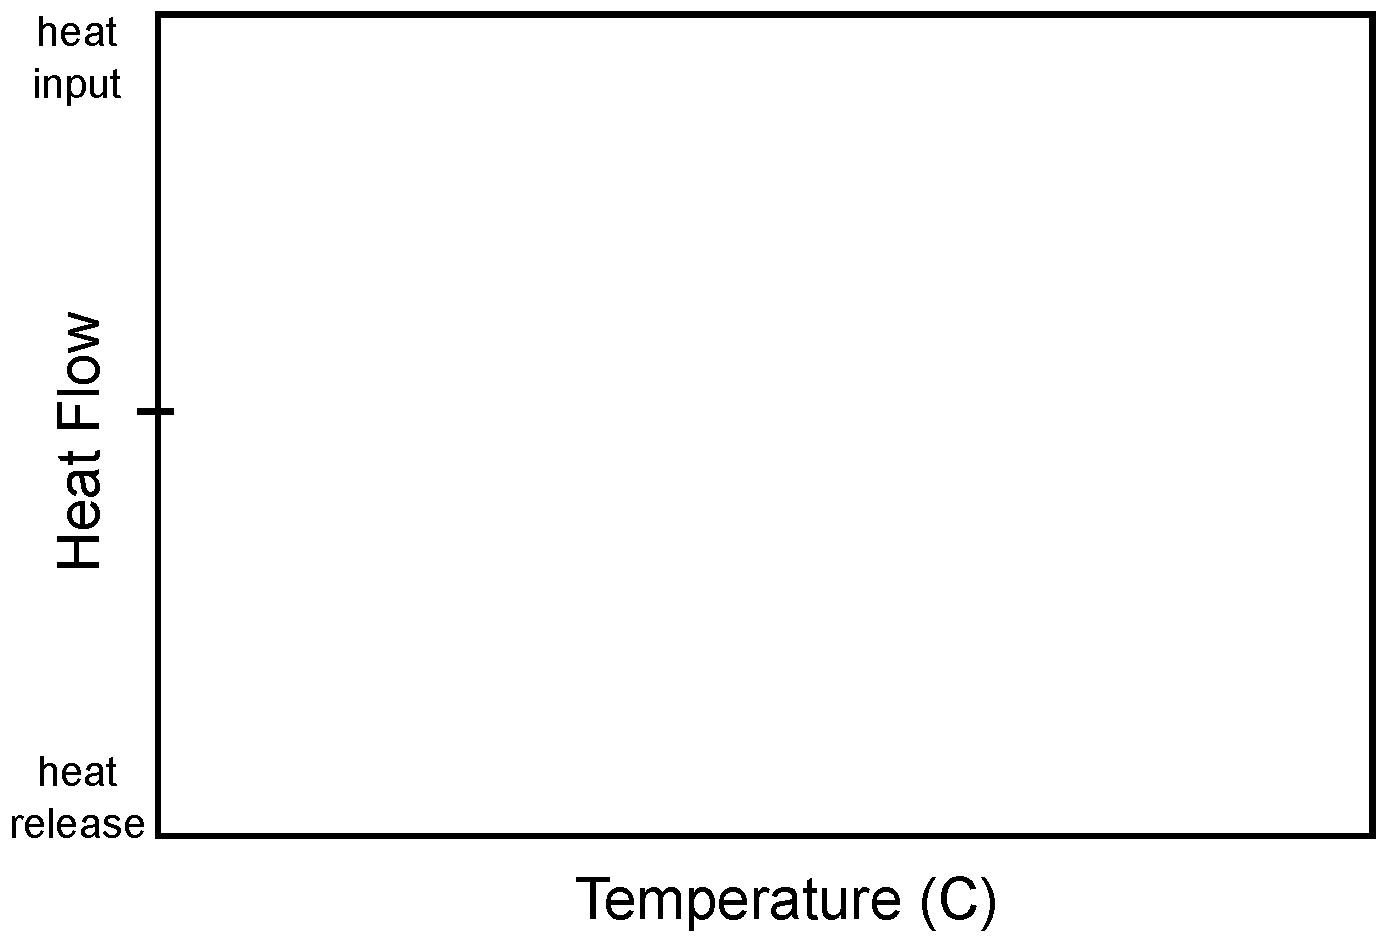
\includegraphics[width=0.5\textwidth]{\figpath/Model2_blankaxes}}
		
	\question Suppose that at temperature $T_0$, a significant amount of heat must be input to break apart some type of intermolecular interaction before the temperature of the sample can keep increasing.  What shape would you expect the resulting DSC curve to have?  Sketch your group's answer on the axes below:\label{\labelbase:ctq:delHtrans}
	
		\vspace{6pt}
		\centerline{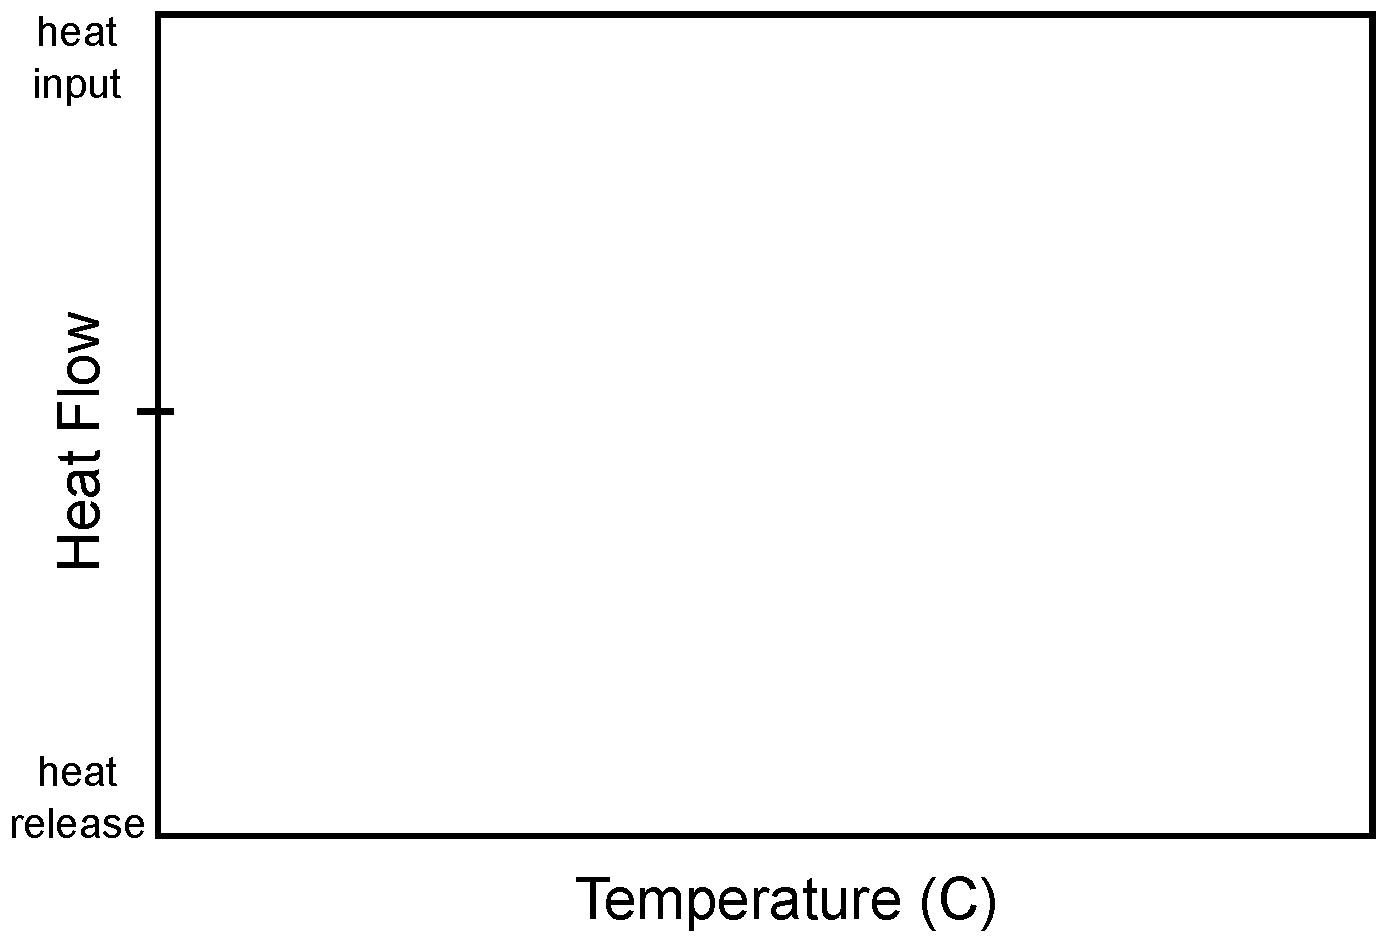
\includegraphics[width=0.5\textwidth]{\figpath/Model2_blankaxes}}
		
	\question Which of the two cases sketched above (CTQ \ref{\labelbase:ctq:CPincrease} or CTQ \ref{\labelbase:ctq:delHtrans}) do you expect to best describe the \emph{melting transition} of a crystalline polymer?  Briefly explain your group's reasoning in 1-2 complete sentences.
	
		\begin{solution}[2in]
		\end{solution}
	
	\question Which of the two cases sketched above do you expect to best describe the \emph{glass transition} of a glassy polymer?  Briefly explain your group's reasoning in 1-2 complete sentences.
	
		\begin{solution}[2in]
		\end{solution}
	
	\question Sketch the shape of the DSC curve you would expect to measure for a polymer that has \emph{both} a glass transition \emph{and} a melting transition on the axes below:
	
		\vspace{6pt}
		\centerline{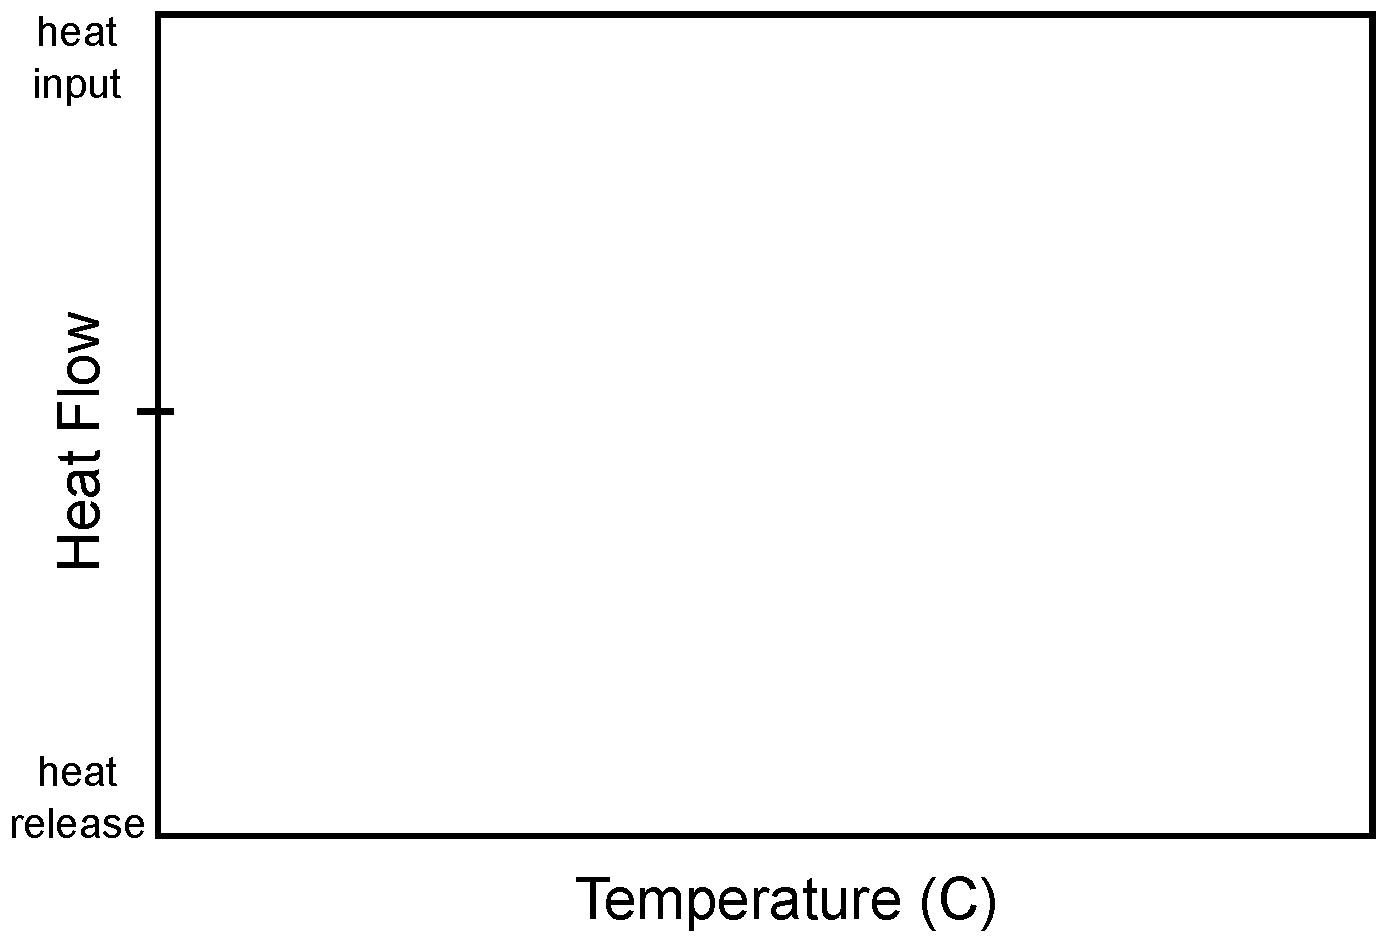
\includegraphics[width=0.5\textwidth]{\figpath/Model2_blankaxes}}
	
	\clearpage
	\question A DSC trace measured for polyethyleneterephthalate (PET) is shown below:
	
		\vspace{6pt}
		\centerline{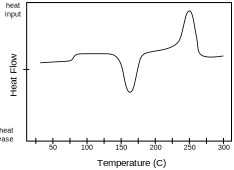
\includegraphics[width=0.5\textwidth]{\figpath/Model2_PET}}
	
		\begin{enumerate}
			\item What is the glass transition temperature for this material?
			
				\begin{solution}[0.5in]
				\end{solution}
			
			\item What is the melting temperature for this material?
			
				\begin{solution}[0.5in]
				\end{solution}
			
			\item Are there any unexpected features in this curve? If so, what do the sign and shape of these feature(s) suggest about the process(es) they might represent?
			
				\begin{solution}[2in]
				\end{solution}
		\end{enumerate}
	
\end{ctqs}





%\begin{exercises}

%	\exercise \dogts
	
%\end{exercises}


%\begin{problems}
%
%	\problem First exercise
%	\problem Second exercise
%	
%\end{problems}


	
\end{activity}